\documentclass[slovene,11pt,a4paper]{article}
\usepackage[margin=2cm,bottom=3cm,foot=1.5cm]{geometry}

\setlength{\parindent}{0pt}
\setlength{\parskip}{0.5ex}
\pagestyle{empty}

\usepackage[pdftex]{graphicx}
\graphicspath{{figs/}}

\DeclareGraphicsExtensions{.pdf,.png}
\usepackage{amsmath}
\usepackage{amsfonts}
\usepackage{mathrsfs}
\usepackage[usenames]{color}
\usepackage[slovene]{babel}
\usepackage[utf8]{inputenc}
\usepackage{siunitx}


%\usepackage[greek,slovene]{babel}
%\usepackage[T1]{fontenc}
%\usepackage{fullpage}

\usepackage{subfig}
\usepackage{xspace}
\usepackage{parskip}
\usepackage{hyperref}
\usepackage{tgschola}

%
\newcommand{\logl}{\ensuremath{\mathrm{ln}\mathcal{L}\!}}
%
\title{
\sc\large Praktikum strojnega učenja\\
\bigskip
\bf\Large 1.~naloga\\ Modeliranje 1-D porazdelitev: Razpadi Higgsovega bozona
}
\author{}
\date{}


\begin{document}
\maketitle
\vspace{-1cm}
V prvem obdobju delovanja (t.i. obdobje ``Run 1'', 2009-2013) Velikega hadronskega trkalnika (Large Hadron Collider, LHC) v Evropskem laboratoriju za jedrske raziskave CERN (Conseil Europeen pour la Recherche Nucleaire), ki se nahaja blizu Ženeve v Švici, sta eksperimenta ATLAS in CMS julija 2012 neodvisno odkrila tudi Higgsov bozon, zadnji še neodkriti delec v napovedih Standardnega modela \cite{atlas-hig,cms-hig}.

V letih 2015-2018 (obdobje ``Run 2'') je nato LHC obratoval pri novi rekordni težiščni energiji trkov protonov $\sqrt{s} = $ 13 TeV, kar imenujemo obdobje ``Run 2'' delovanja LHC. Pri meritvi podatkov iz tega obdobja, ob približno petkrat več izmerjenih trkih in skoraj dvakrat večji težiščni energiji kot v ``Run 1'', se kolaboracije na LHC posvečajo iskanju naravnih zakonov onkraj Standardnega modela ter natančni meritvi napovedi Standardnega modela, zlasti lastnosti Higgsovega bozona. 


Iskanje \textbf{signala} (zanimivih, a redkih procesov) v tolikšni količini podatkov je vedno velik izziv, saj so le-ti praviloma težko ločljivi od dominantnih procesov \textbf{ozadja} (t.j. že znanih in izmerjenih interakcij med delci). Kljub uporabi najnaprednejših računskih metod za ločevanje procesov signala od ozadja (na primer Deep Neural Networks, Boosted Decision Trees in druge metode strojnega učenja), je delež procesov ozadja v končnih vzorcih praviloma še vedno zelo velik. Tako je zelo pomembno, da lahko kinematične porazdelitve tega ozadja čim bolj natančno opišemo, da ga lahko nato učinkovito `odštejemo' od podatkov (in kar ostane je možen iskani signal). Pri tem si pomagamo z računalniškimi simulacijami procesov ozadja, ki pa jih nato poskušamo še dodatno izboljšati. Reprezentativen primer, kjer velikost ozadja za rede velikosti presega napoved signala je podan na sliki \ref{fig:primer}.
\begin{figure}[hbt]
\centerline{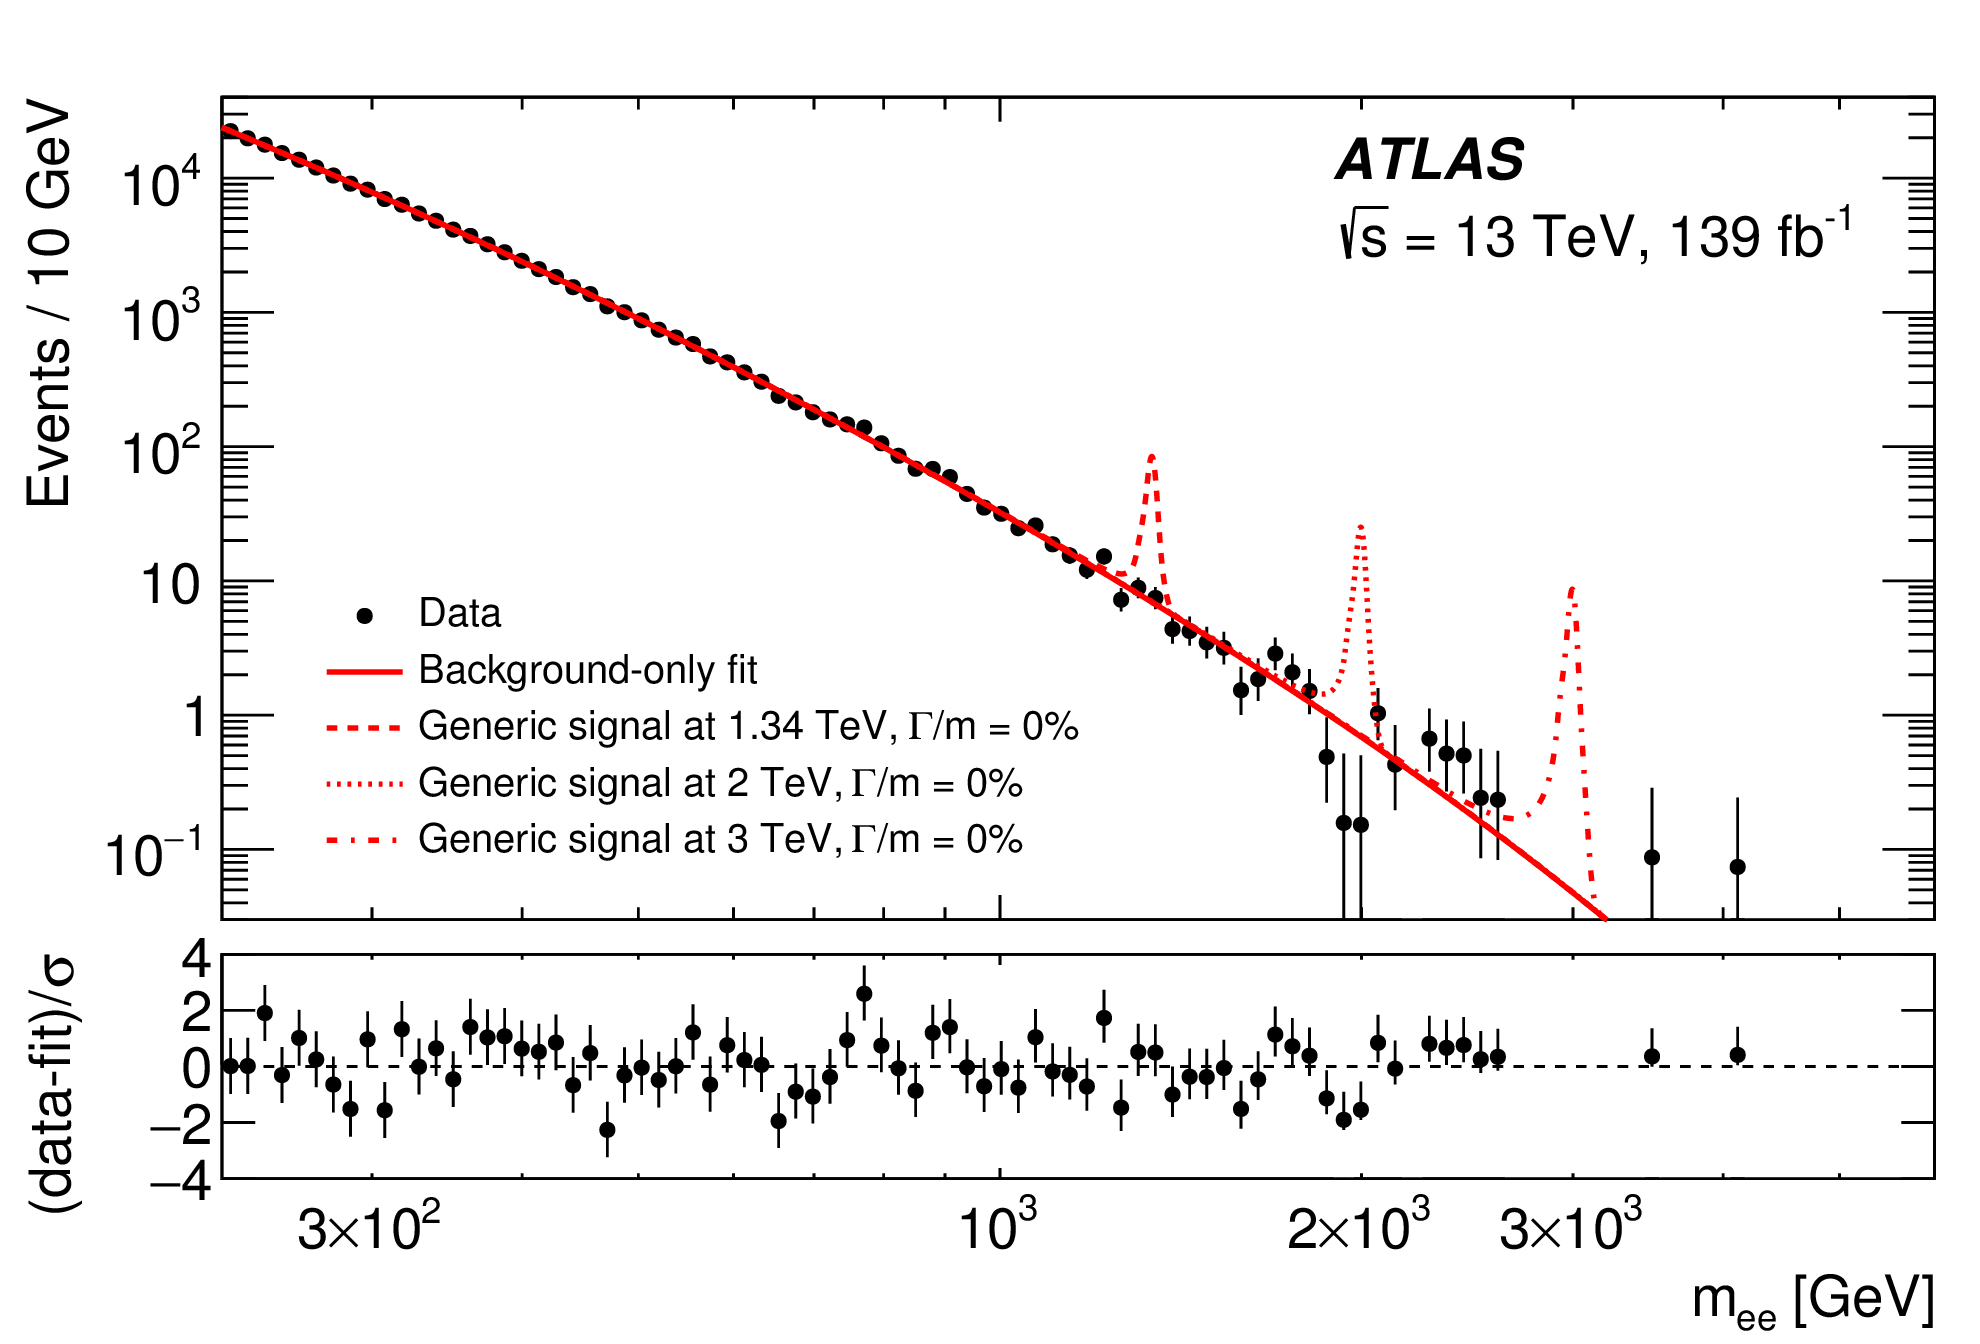
\includegraphics[width=0.6\linewidth]{mee.png}}
\caption{Porazdelitev izmerjenih dogodkov po rekonstruirani invariantni masi dveh izbranih elektronov ($m_{ee}$) z napovedjo ozadja in signala. Napoved ozadja je potrebno čez več velikostnih redov interpolirati v območje iskanega signala. Vzeto iz meritve kolaboracije ATLAS \cite{atlas-mee}.}
\label{fig:primer}
\end{figure}



Ker gre pri (simuliranem ali pravem) nastanku procesov signala in ozadja za statistične procese, so rezultati meritev poleg merskih napak obremenjeni s statistično nedoločenostjo. Statistično napako simuliranih procesov si želimo seveda čim bolj zmanjšati, vendar pa so postopki simulacij računsko zelo zahtevni in tako v praksi nimamo na voljo potrebnih milijard simuliranih trkov procesov ozadja, ki bi nam podali zanemarljivo statistično napako. Simulacije same tudi zaradi nepopolnega opisa (modeliranja) fizikalnih procesov v vseh primerih ne opišejo merjenih podatkov z zadovoljivo natančnostjo. 

Pri `končnem' opisu procesov ozadja si tako pomagamo z regresijo (`fitom', parametrizacijo) kinematičnih porazdelitev, ki nas zanimajo - tipično je to eno-dimenzionalna porazdelitev kinematične količine, ki najbolje loči med signalom in ozadjem. Postopek regresije ozadja nato izhaja ali iz simuliranih porazdelitev ali iz predpostavljenih (po možnosti fizikalno motiviranih) funkcijskih oblik, ki jih poskušamo dodatno prilagoditi podatkom v kinematičnem območju porazdelitve, kjer signala ne pričakujemo (t.i. `sideband') in jih nato ekstrapoliramo v signalno območje. 

Pri tem je bistveno poudariti, da kot fiziki predpostavimo, da so `prave' porazdelitve ozadja (in signala) \emph{gladke} verjetnostne porazdelitve s fizikalno motiviranimi (razumljivimi) variacijami oblike (torej ekstremi - `vrhovi', prevojne točke ipd.). Tu torej ne gre za to, da bi poiskali funkcijo, ki `pofita' vse merske vrednosti - kar bi lahko dosegli že s polinomom dovolj visokega reda, temveč gre tu v resnici za kombinacijo \emph{glajenja} (ang. `smoothing') in popravkov predpostavljene funkcijske oblike za najboljše ujemanje s podatki. 
\begin{figure}[tb]
\begin{center}
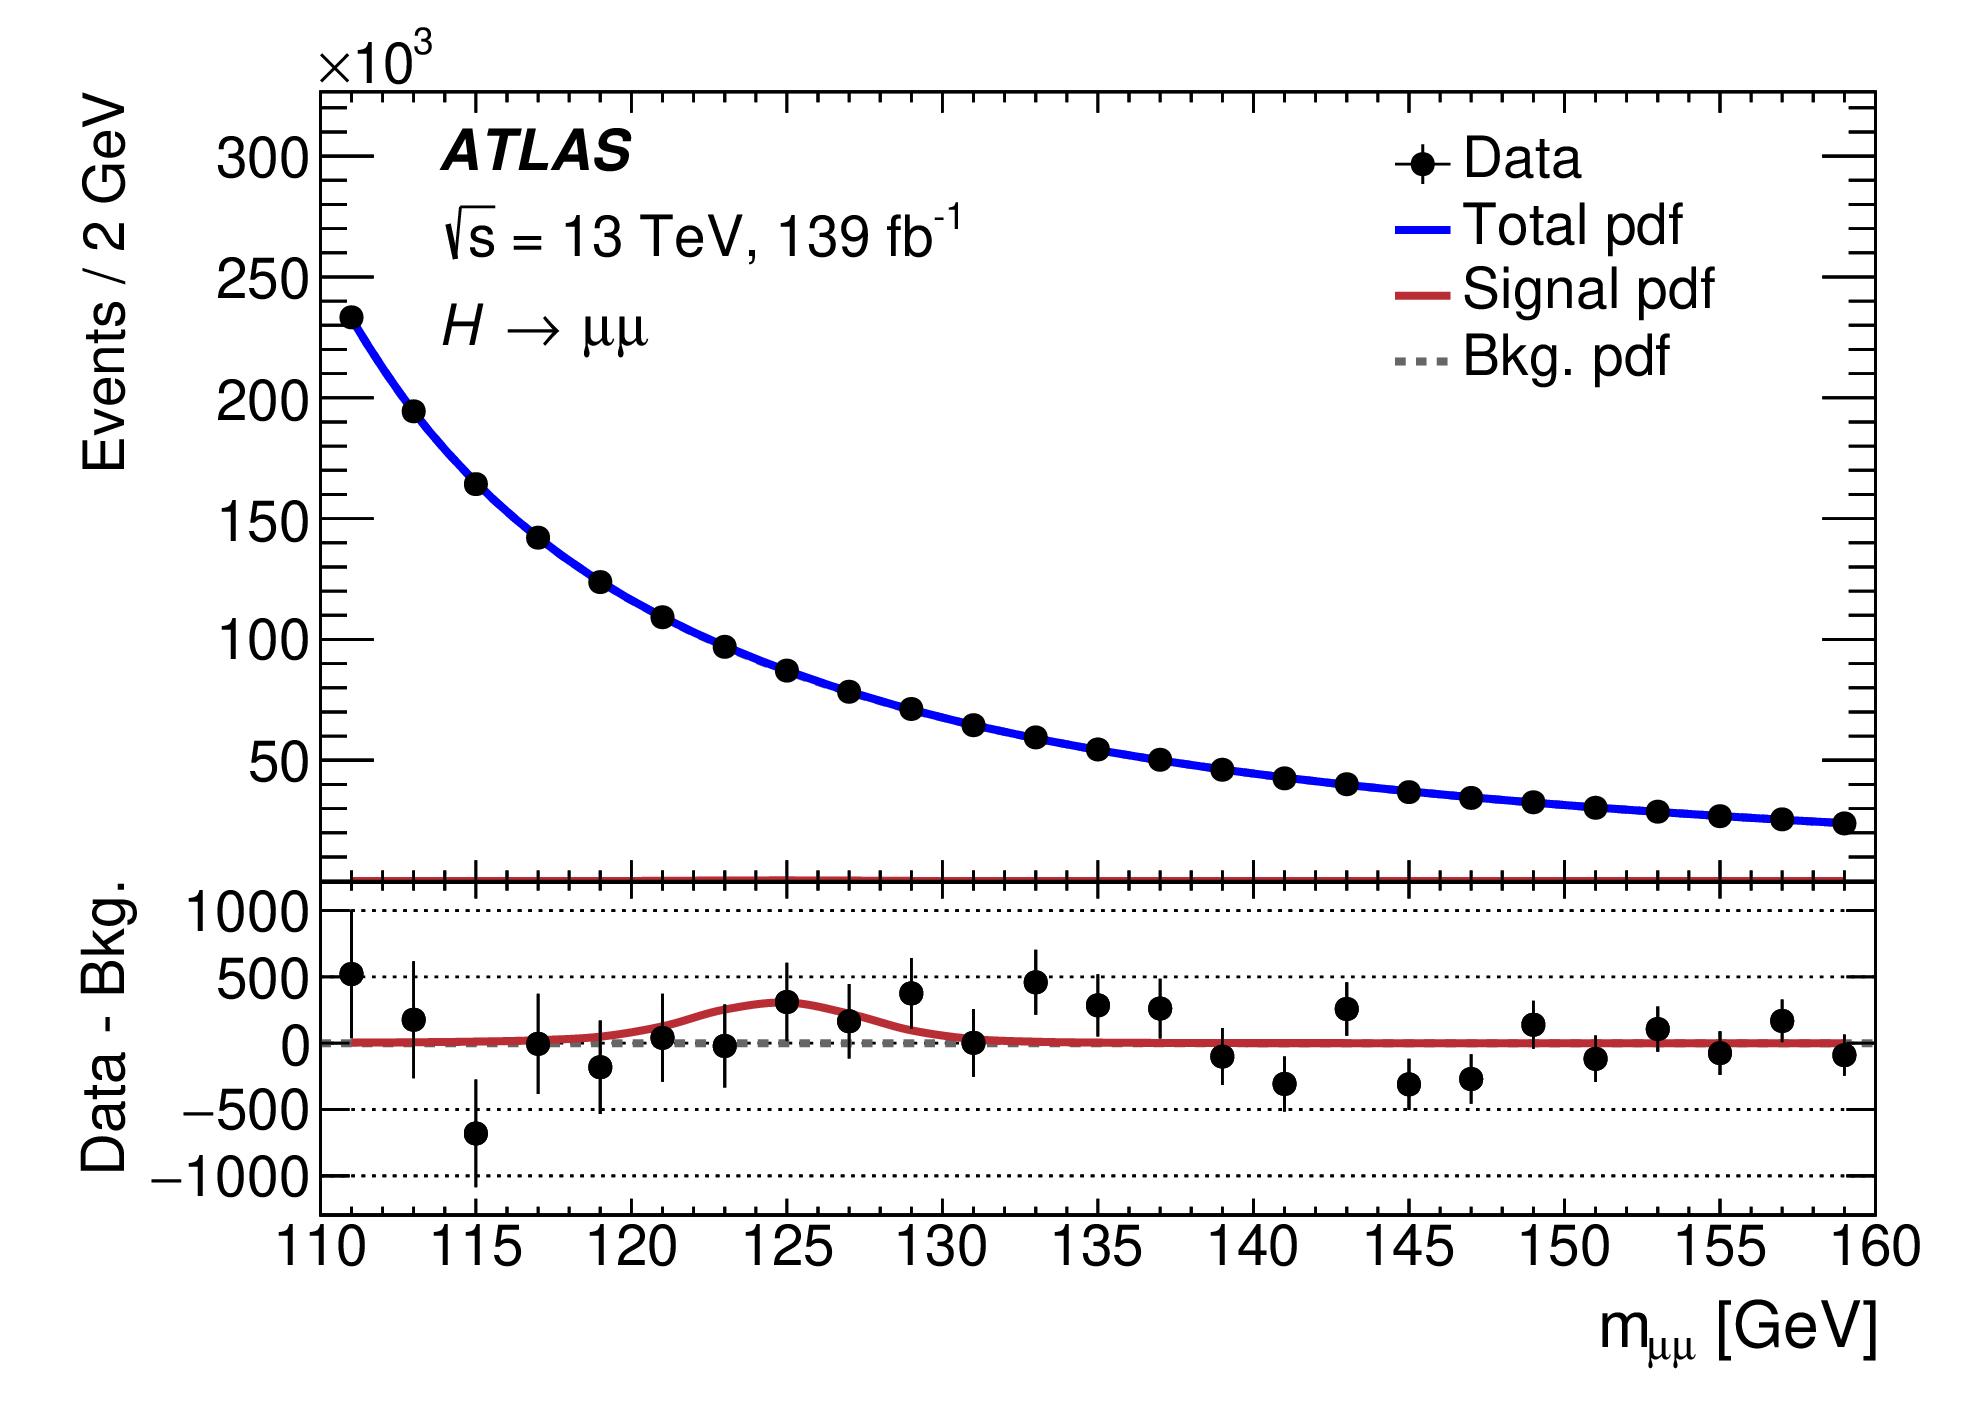
\includegraphics[width=0.45\textwidth]{hmumu-atlas.png} 
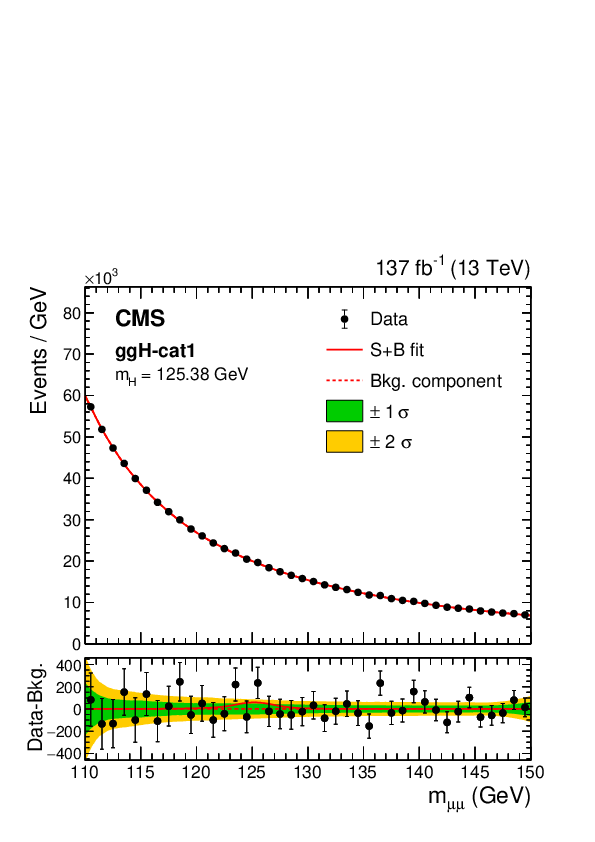
\includegraphics[width=0.45\textwidth]{hmumu-cms.png} 
\end{center}
\caption{Porazdelitev izmerjenih dogodkov po rekonstruirani invariantni masi dveh izbranih mionov ($m_{\mu\mu}$), objavljena rezultata kolaboracij ATLAS \cite{atlas} in CMS \cite{cms}. Vzeto iz navedenih člankov.}
\label{fig:meas}
\end{figure}

Metode regresije so danes pomemben element metod strojnega učenja, kjer poskušamo iz omejene količine podatkov (tudi, če je ta velikanska na absolutni skali) izvleči čim več informacij o samem procesu. Poleg tega lahko tu prvič v praksi srečamo korake in koncepte, ki so prisotni povsod v strojnem učenju, kot so funkcija cene/izgube (`cost/loss' function), postopki minimizacije neznanih parametrov s pomočjo le-te in gradientnih metod, kot tudi probleme neuspešnega modeliranja (`over/under-fitting') ipd. 

V našem primeru linearna regresija seveda ne bo dovolj, lahko prilagajamo različne funkcijske oblike ali pa, v smeri naprednejših ML metod, uporabimo metode podpornih vektorjev (Support Vector Machines (SVM) Regression) in jeder (ang. kernel), ki nam naredijo preslikavo iz linearnega nabora parametrov v nelinearni več-dimenzionalni (tudi neskončno) prostor parametrov in tako omogočajo veliko fleksibilnost regresije. Z dodatkom Bayesove teorije verjetnosti in statistično re-interpretacijo naših postopkov pridemo tudi iz regresije z uporabo gausovskih jeder do regresije z gausovskimi procesi Gaussian Process Regression, GPR), ki nam omogočajo elegantno (algebraično) oceno nedoločenosti/razmazanosti dobljenih funkcij, kar je pri minimizaciji parametrov v funkciji izgube tipično numeričen dodatek z različno kvaliteto implementacij, ker ne predpostavi Gaussove oblike rezultata (dober zgled je CERNov paket za minimizacijo MINUIT).

Poleti leta 2020 sta kolaboraciji ATLAS in CMS objavili novi meritvi iskanja (redkega) razpada Higgsovega bozona v dva miona (H$\to \mu^+\mu^-$) \cite{atlas,cms}. Objavljeni izmerjeni porazdelitvi sta prikazani na sliki \ref{fig:meas}. V dani nalogi bomo obravnavali (poenostavljeno) meritev eksperimenta ATLAS, kjer si bomo ogledali kinematično porazdelitev dogodkov po rekonstruirani invariantni masi dveh izbranih mionov ($m_{\mu\mu}$), kot to prikazuje slika \ref{fig:m_mumu}. Glavni proces ozadja je razpad šibkega bozona Z$\to\mu^+\mu^-$, ki prispeva resonančno porazdelitev z vrhom pri ($m_\mathrm{Z}$ = 91 GeV\footnote{Uporabljamo enote $\hbar=c_0=1$.}), kjer pa se rep invariantne mase razširi tudi precej nad maso Higgsovega bozona ($m_\mathrm{H}$ = 125 GeV). Kot lahko vidimo, nam da ta proces ozadja za več redov velikosti več dogodkov, kot jih pričakujemo iz signalnega razpada Higgsovega bozona. K ozadju prispevajo v manjši meri tudi mnogi drugi procesi, kot so tvorba in razpad parov šibkih bozonov ($ZZ$, $WW$, $WZ$), nastanek in razpad kvarkov top itd\ldots. 

Za nalogo so na razpolago simulirani in izmerjeni dogodki kolaboracije ATLAS, dejansko uporabljeni v dani analizi, podajajo pa vrednost $m_{\mu\mu}$, ki je potrebna za zadano nalogo. Za vsak dogodek je podana tudi utež, ki je za podatke enaka 1, v primeru simulacije pa predstavlja nabor merskih popravkov in obenem reskalira dogodke tako, da je vsota uteži enaka pričakovani vrednosti števila izmerjenih dogodkov za vključene procese ($\sum wt = N_{\mathrm{proc}}$). Celotna statistična napaka je potem ($\sigma=\sqrt{\sum wt^2}$). To za simulacijo pomeni, da napaka ni Poissonova, ker gre tu za preuteženo normirano distribucijo (število dogodkov v simulaciji je mnogo večje od pričakovane vrednosti števila izmerjenih dogodkov za proces $N_{\mathrm{MC}} >> N_{\mathrm{proc}}$). Uporaba $\sigma= \sqrt{N_{\mathrm{proc}}}$ je torej za simulacijo zelo narobe! Analogno seveda velja tudi za vsak `predal' (ang. `bin'), ko dogodke razvrstimo v histogram). 
\begin{figure}[tb]
\begin{center}
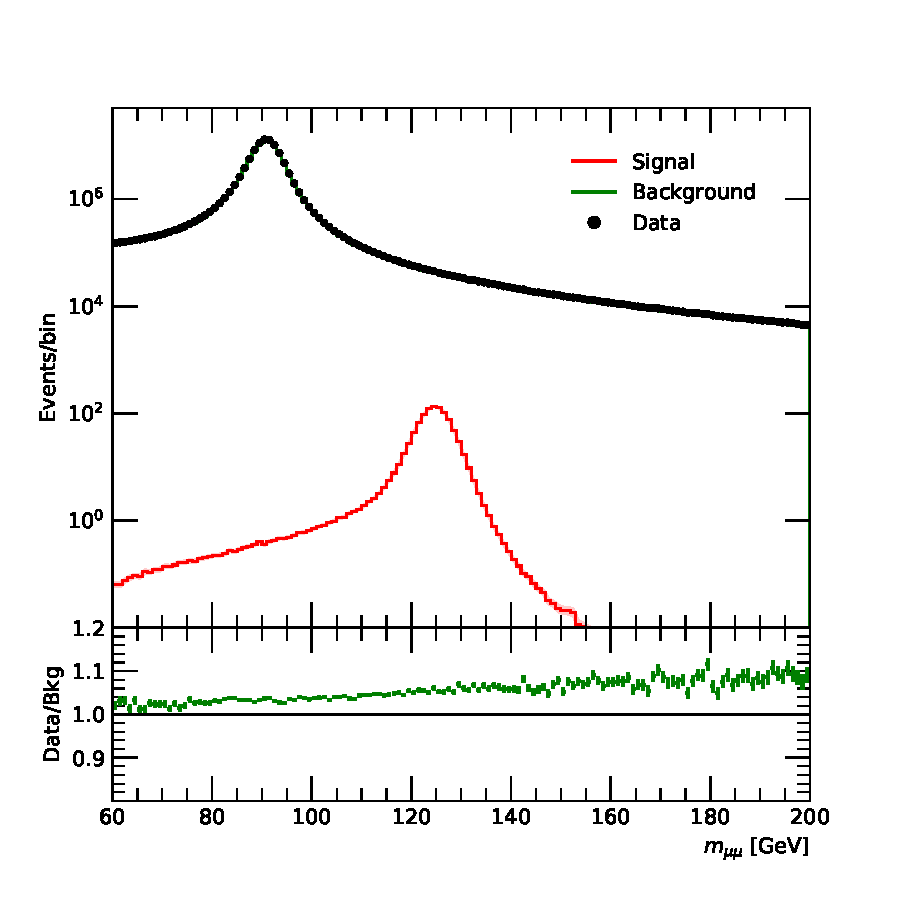
\includegraphics[width=0.33\textwidth]{all_hmumu_ratio.pdf} \hspace*{-0.6cm}
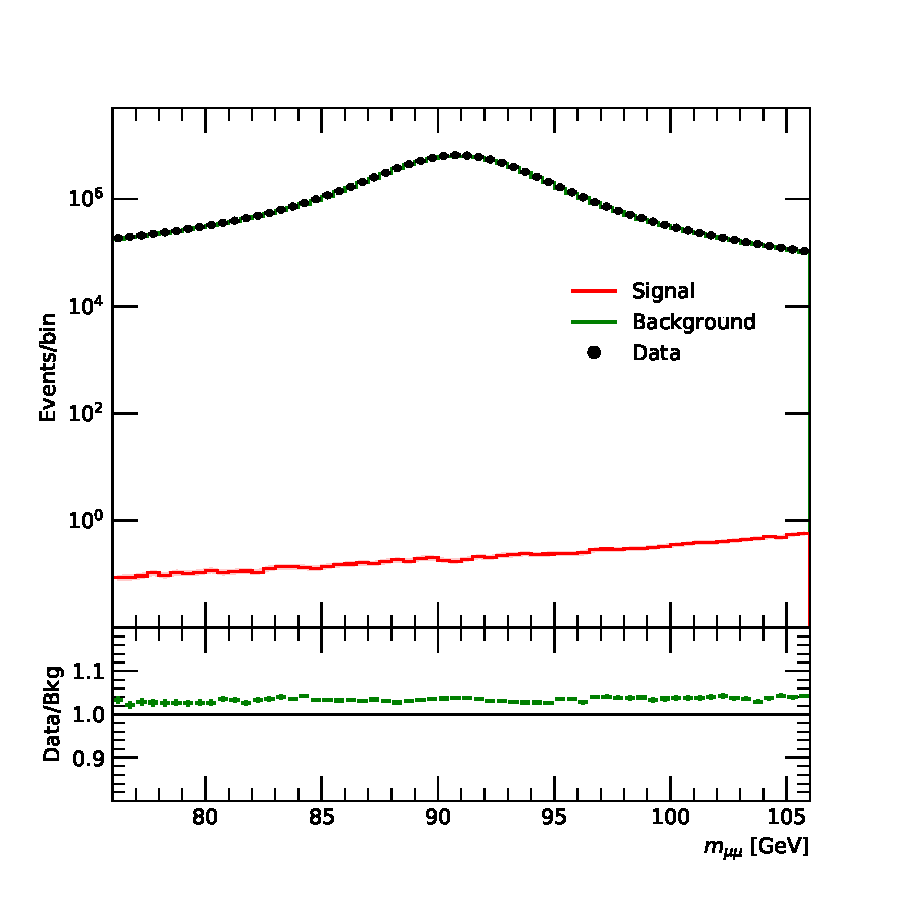
\includegraphics[width=0.33\textwidth]{zpeak_hmumu_ratio.pdf} \hspace*{-0.6cm}
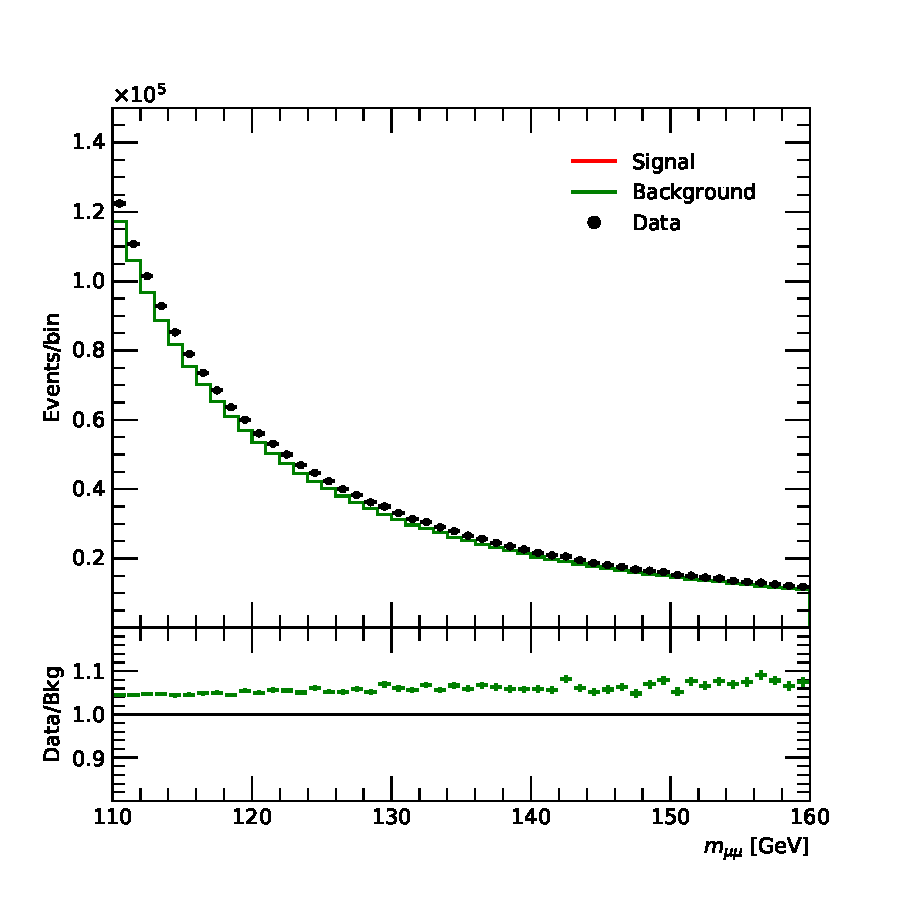
\includegraphics[width=0.33\textwidth]{higgs_hmumu_ratio.pdf} 
\end{center}
\caption{Porazdelitev izmerjenih in simuliranih dogodkov po rekonstruirani invariantni masi dveh izbranih mionov ($m_{\mu\mu}$). Reproducirano iz podatkov kolaboracije ATLAS. Levo: porazdelitev po celotnem intervalu ([60 GeV, 200 GeV], št. predalov=140), sredina: porazdelitev na intervalu okoli mase bozona $Z$ ([76 GeV, 106 GeV], št. predalov=60) in desno: porazdelitev bližje masi higgsovega bozona ([110 GeV, 160 GeV], št. predalov=50).}
\label{fig:m_mumu}
\end{figure}

Kot lahko vidimo že iz slike \ref{fig:m_mumu}, je ujemanje simulacije z izmerjenimi podatki v območju [110 GeV, 160 GeV], kjer iščemo razpad Higgsovega bozona, nezadovoljivo. Signal lahko za potrebe določitve ozadja omejimo na primer na območje [120 GeV, 130 GeV], ozadje tako lahko varno primerjamo s podatki na preostalem območju (te meje lahko tudi še sami optimiziramo, po potrebi). Na voljo imamo cel šop metod za ustrezno določitev ozadja:
\begin{itemize}
\item Popravimo napoved simulacije tako, da jo dodatno korigiramo (utežimo) s polinomom dovolj nizkega reda.
\item Uporabimo teoretično motivirane nastavke za modeliranje oblike porazdelitve ozadja. Cel kup nastavkov je na voljo v publikaciji kolaboracije ATLAS \cite{atlas-bkg}. Analiza kolaboracije CMS tako uporabi: 
\begin{equation*}
\operatorname{mBW}\left(m_{\mu \mu} | m_\mathrm{Z}, \Gamma_\mathrm{Z}, a_{1}, a_{2}, a_{3}\right)=\frac{\mathrm{e}^{a_{2} m_{\mu \mu}+a_{3} m_{\mu \mu}^{2}}}{\left(m_{\mu \mu}-m_{\mathrm{Z}}\right)^{a_{1}}+\left(\Gamma_{\mathrm{Z}} / 2\right)^{a_{1}}},
\end{equation*}
kjer sta $\Gamma_\mathrm{Z}$ = 2.49 GeV in $m_\mathrm{Z}$ = 91.19 GeV razpadna širina in masa bozona $Z$, parametri $a_{i}$ pa so prosti parametri za prilagajanje funkcije podatkom. Kolaboracija ATLAS uporabi precej bolj komplicirano teoretično formulo, ki je na voljo na spletni učilnici v Python kodi.
\item Uporabimo SVM metode z različnimi jedri in regularizatorji (Kernel Ridge Regression, KRR).
\item Uporabimo metodo strojnega učenja, t.j. gaussovskih procesov (Gaussian Process Regression, GPR), ki temelji na različnih jedrih. Posebna oblika Gibbsovega jedra je na voljo na spletni učilnici, lahko jo uporabite tudi za KRR. 
\item Uporabimo dekompozicijo na ortogonalne polinome (Functional Decomposition, FD), na primer eksponentne polinome, razvite prav v ta namen\cite{FD-regression}.
\end{itemize}
Pri določitvi prostih parametrov pri lepljenju (fitanju) na podatke je zaradi statistične narave podatkov v histogramu naša funkcija izgube kar minus (logaritem) funkcije maksimalne zanesljivosti (-\logl ), določena s Poissonovo verjetnostjo za vsak predal (`bin') v histogramu:
\begin{equation}
-\logl(\vec{N}|\vec{\alpha}) = -\ln\left(\prod\limits_{k=1}^{n_\mathrm{bins}} P(N_k|\mu_k(\vec{\alpha}))\right) = \sum\limits_{k=1}^{n_\mathrm{bins}} -N_k\ln\mu_k(\vec{\alpha})-\mu_k(\vec{\alpha})+\ln N_k! ~, 
\end{equation}
kjer so $N_k$ vrednosti podatkov v predalih histograma in $\mu_k$ pričakovane vrednosti. Slednje vsebujejo naš model ozadja (in/ali signala) ter neznane parametre $\vec{\alpha}$, ki jih prilagajamo z minimizacijo -\logl. Pri dovolj velikih vrednostih $N_k$, je dovolj dober približek Poissonove porazdelitve z Gaussovo in potem dobimo:
 \begin{equation}
-\logl(\vec{N}|\vec{\alpha}) \simeq - \sum\limits_{k=1}^{n_\mathrm{bins}} \frac{(N_k-\mu_k(\vec{\alpha}))^2}{\mu_k} ~, 
\end{equation}
kjer lahko prepoznamo obliko izraza za izračun $\chi^2$ s $\sigma_k^2=\mu_k$. Če bi napake (variance) $\sigma^2_k$ ne poznali, oziroma bi predpostavili, da je konstantna, bi iz izraza za \logl~ lahko napako izpustili in dobili eno najbolj pogostih funkcij izgube v strojnem učenju, MSE($\vec{\alpha}$) = $\sum(N_k-\mu_k(\vec{\alpha}))^2$ (v komercialni rabi strojnega učenja merske napake niso znane ali pa niso zanimive). 


Za parametrizacijo signala se tipično uporabi t.i. Crystal Ball (CB) oblika funkcije, ki je kombinacija Gaussovega jedra in debelejših repov:
\begin{equation*}
\operatorname{CB}\left(m_{\mu \mu}|\alpha_{\mathrm{L},\mathrm{R}},n_{\mathrm{L},\mathrm{R}}, m_{\mathrm{CB}},\sigma_{\mathrm{CB}} \right)=\left\{\begin{array}{l}
\mathrm{e}^{-\left(m_{\mu \mu}-m_{\mathrm{CB}}\right)^{2} / 2 \sigma_{\mathrm{CB}}^{2}}, \quad-\alpha_{\mathrm{L}}<\frac{m_{\mu \mu}-m_{\mathrm{CB}}}{\sigma_{\mathrm{CB}}}<\alpha_{\mathrm{R}} \\
\left(\frac{n_{\mathrm{L}}}{\left|\alpha_{\mathrm{L}}\right|}\right)^{n_{\mathrm{L}}} \mathrm{e}^{-\alpha_{\mathrm{L}}^{2} / 2}\left(\frac{n_{\mathrm{L}}}{\left|\alpha_{\mathrm{L}}\right|}-\left|\alpha_{\mathrm{L}}\right|-\frac{m_{\mu \mu}-m_{\mathrm{CB}}}{\sigma_{\mathrm{CB}}}\right)^{-n_{\mathrm{L}}}, \frac{m_{\mu \mu}-m_{\mathrm{CB}}}{\sigma_{\mathrm{CB}}} \leq-\alpha_{\mathrm{L}} \\
\left(\frac{n_{\mathrm{R}}}{\left|\alpha_{\mathrm{R}}\right|}\right)^{n_{\mathrm{R}}} \mathrm{e}^{-\alpha_{\mathrm{R}}^{2} / 2}\left(\frac{n_{\mathrm{R}}}{\left|\alpha_{\mathrm{R}}\right|}-\left|\alpha_{\mathrm{R}}\right|+\frac{m_{\mu \mu}-m_{\mathrm{CB}}}{\sigma_{\mathrm{CB}}}\right)^{-n_{\mathrm{R}}}, \frac{m_{\mu \mu}-m_{\mathrm{CB}}}{\sigma_{\mathrm{CB}}} \geq \alpha_{\mathrm{R}}
\end{array}\right.
\end{equation*}
Ker so prosti parametri $N_{L,R}$ in $\alpha_{L,R}$ visoko korelirani je za hitro konvergenco regresije (fita, minimizacije) smiselno kombinirati samo minimizacijo s `pregledom' (scanning), namreč da spreminjamo vrednosti $n_{L,R}$ po neki mreži smiselnih vrednosti in poiščemo $\alpha_{L,R}$ z minimizacijo in nato (iterativno) obrnemo postopek in `skeniramo' $\alpha_{L,R}$ in minimiziramo $n_{L,R}$ - kar je uporabna vaja, ker je to pogost postopek za nestabilne minimizacije \ldots
Za vajo uporabi dani nastavek za regresijo na simulirani napovedi za signal. Nastavek za prilagajanje parametrične napovedi je potem oblike:
\begin{equation*}
-\ln\mathcal{L}(\vartheta) = \sum_{k=1}^M \frac{(\mu_k-f(x_k|\vartheta))^2}{\sigma_{\mu_k}^2},
\end{equation*}
kjer je, kot že rečeno, pričakovano število dogodkov v predalu $k$ podano z $\mu_k=\sum_{x \in k} wt$, napaka na napovedi signala $\sigma_{\mu_k}$ podana z vsoto kvadratov vseh uteži dogodkov v predalu $\sigma_{\mu_k}=\sqrt{\sum_{x \in k} wt^2}$.
% z binomsko (multinomsko) napako:
% \begin{equation*}
% \sigma_{\mu_k} = \alpha_k\sqrt{ \frac{N_k(N_{\text{exp}}-N_k)}{N_{\text{exp}}^3}} = \sqrt{\sum_{x \in k} wt^2}
% \end{equation*}
% Tu je $\alpha_k$ normalizacijski koeficient (dobljen teoretično ali eksperimentalno s fitom na podatke), $N_k$ je število simuliranih dogodkov v k-tem predalčku in $N_{\text{exp}}$ je celotno število v vseh predalčkih. 
Pri delu se tudi \emph{namenoma zmoti} pri določanju napake na vrednostih v histogramu, uporabi napačno Poissonsko formulo ($\sigma_{\mathrm{N_k}}=\sqrt{N_\mathrm{k}}$)) ali pa konstantno napako (velike in male vrednosti) in preveri učinek. Enako velja seveda za parametrizacijo simulacije ozadja.

Končni korak naloge je, da od podatkov odšteješ končno napoved ozadja (v histogramih) in pogledaš kaj ostane, oziroma, koliko signala bi lahko izluščil pri različnih metodah (lahko prešteješ dogodke v predalčku pri 125 GeV ali, še bolje, uporabiš regresijo/fit za normalizacijo CB oblike signala na podatkih). Signal nalepiš na dobljeni histogram tako, da dodaš kot prost parameter normalizacijo CB funkcije in jo optimalno prilepiš (spet fit) na podatke v relevantnem območju signala (lahko malo eksperimentiraš z mejami le-tega). Zaželjeno je, da dobiš tudi napako tega fita. Primerjaj, kaj dobiš za različno zglajeno ozadje.

V dokumentu o modeliranju ozadij kolaboracije ATLAS \cite{atlas-bkg} je tudi nabor sofisticiranih metod, ki jih v praksi uporabimo za preverjanje naših napovedi ozadja (npr. `spurious signal method'), ki pa jih bralec lahko uporabi le po želji - so pa priporočeno branje za kdaj kasneje v bralčevi karieri\ldots


\section*{Navodila in usmeritve}
V nadaljevanju sledijo podrobnejša navodila in usmeritve za lažje reševanje naloge.
\begin{enumerate}
    \item \label{item:hist} Iz surovih (`raw') podatkov zgeneriraj svoje histograme s pomočjo predpripravljene skripte \texttt{create\_histograms.py}, pri kateri lahko spreminjaš število predalov (``bin''-ov) in $m_{\mu \mu}$ interval, ki ga boš opazoval/-a. Histogrami (mejne in sredinske $x$ vrednosti predalov, vrednosti in napake) se shranijo v formatu \texttt{.npz}.
    \item \label{item:visual} Ko imaš zgenerirane svoje histograme, jih lahko izrišeš s pomočjo skripte \texttt{visualize\_data.py} (ustrezno s točko \ref{item:hist} spremeni ime datotek, ki jih nalagaš).
    \item \label{item:error} Preveri, če so napake res pravilno upoštevane. Lahko jih namenoma pokvariš in ponoviš prva dva koraka, da vidiš vpliv.
    \item \label{item:simBkg} Da se spoznaš z osnovnim fitanjem, najprej zgladi histogram simuliranega ozadja (``simulated background'') s pomočjo preprostejših matematičnih funkcij in nadaljuj do različnih teoretično podkrepljenih nastavkov (CMS, ATLAS nastavki). Dobiš funkcijo / vrednosti predalov $m(x_k)$.
    \item \label{item:simSig} Prilagodi funkcijo CB histogramu simuliranega signala, pri čemer upoštevaj še dodatni normalizacijski faktor. Dobiš funkcijo / vrednosti predalov $s(x_k)$.
    \item \label{item:dataBkg} Ker simulacija ozadja ni vedno najboljša, se po navadi za oceno ozadja raje vzame izmerjene podatke, pri čemer pa je potrebno izključiti območje, kjer pričakujemo signal (``blinding'') - nočemo fitati še signala! Prilagodi torej funkcijo histogramu podatkov, da dobiš dobro oceno za ozadje (``background from data'') in pri tem pazi, da pri fitu \textbf{ne} upoštevaš območja okrog mase Higgsovega bozona, npr. izključi interval 120 - 130 GeV. Dobiš funkcijo / vrednosti predalov $b(x_k)$.
    \item \label{item:extSig} Od podatkov odštej čim bolje zglajeno ozadje, ki si ga dobil/-a v prejšnji točki \ref{item:dataBkg}, da dobiš ekstrahiran signal. Če so vrednosti podatkov $d(x_k)$, dobimo ekstrahiran signal $y(x_k)$ kot $y(x_k) = d(x_k) - b(x_k)$.
    \item \label{item:final} Na ekstrahiran signal fitaj CB funkcijo s prostimi parametri, ki si jih dobil/-a v točki \ref{item:simSig} tako, da ji v resnici prilagodiš le nov normalizacijski faktor, npr.: $\alpha_{norm.} \times s(x_k)$. Optimalno je, da je le-ta blizu 1.
    \item \label{item:asimov} Ker je izmerjenega signala še zelo malo, predlagamo, da postopek najprej narediš z umetno napihnjenim signalom - le tega množi z nekim faktorjem (npr. $\gamma = 100$) in ga dodaj podatkom ($s_{new}(x_k) = \gamma \times s(x_k)$ in $d(x_k) = d(x_k) + s_{new}(x_k)$). Ker bo signal na ta način lepo izstopal iz ozadja, ga boš lažje izluščil/-a.
\end{enumerate}

\begin{thebibliography}{10}
\bibitem{atlas-mee}
{ATLAS Collaboration}, “Search for High-Mass Dilepton Resonances Using 139 fb-1 of pp Collision Data Collected at sqrt(s)=13 TeV with the ATLAS Detector.” Physics Letters B 796 (2019): 68–87. 

\bibitem{atlas-hig}
{ATLAS Collaboration}, “Observation of a New Particle in the Search for the Standard Model Higgs Boson with the ATLAS Detector at the LHC.” Physics Letters B 716.1 (2012): 1–29. 
\bibitem{cms-hig}
{CMS Collaboration}, “Observation of a New Boson at a Mass of 125 GeV with the CMS Experiment at the LHC.” Physics Letters B 716.1 (2012): 30–61. 
\bibitem{atlas}
{ATLAS Collaboration}, "A search for the dimuon decay of the Standard Model Higgs boson with the ATLAS detector", preprint arXiv:2007.07830 (2020).
\bibitem{cms}
{CMS Collaboration}, "Evidence for Higgs boson decay to a pair of muons",preprint arXiv:2009.04363 (2020).
\bibitem{atlas-bkg}
{ATLAS Collaboration}, Nicholas Berger, "Recommendations for the Modeling of Smooth Backgrounds", ATL-PUB-STAT-2020-01 (2020), na spletni učilnici. 
\bibitem{FD-regression}
Ryan Edgar, Dante Amidei, Christopher Grud, and Karishma Sekhon. "Functional Decomposition: A new method for search and limit setting." Technical Report, University of Michigan, preprint arXiv:1805.04536 (2018).

\end{thebibliography}

\end{document}